\documentclass[tikz]{standalone}

\usepackage[utf8]{inputenc}
\usepackage{amsmath,mathtools,amssymb,physics,cancel,bm}
\usepackage[cal=boondox]{mathalfa}
\usepackage[per-mode=fraction]{siunitx}
\usepackage{cmbright}
\usepackage[T1]{fontenc}
\usepackage{tikz,pgfplots,pgf,pgfplotstable,tikz-3dplot}
\usetikzlibrary{positioning,
                arrows,
                decorations.pathreplacing,
                decorations.text,
                intersections,
                decorations.pathmorphing,
                patterns,
                fit,
                babel,
                angles,
                quotes,
                shapes,
                calc,
                backgrounds,
                3d} 
\pgfplotsset{compat=newest}

\begin{document}
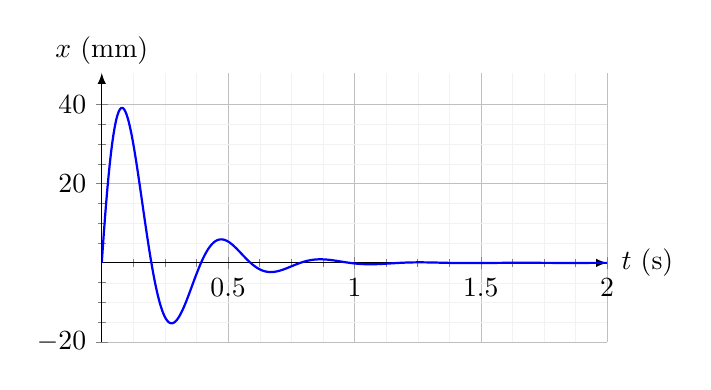
\begin{tikzpicture}
\begin{axis}[
	grid=both,
    grid style={line width=.1pt, draw=gray!10},
    major grid style={line width=.2pt,draw=gray!50},
	xlabel=$t$ (s), 
	ylabel=$x$ (mm), 
	minor tick num=3,
	xmin=0, xmax=2,
	ymin=-20, ymax=48,
	axis lines=middle,
	samples=1000,
	domain=0:2,
	xlabel style={at={(ticklabel* cs:1.15)},anchor=east},
    ylabel style={at={(ticklabel* cs:1.17)},anchor=north},
	axis line style={-latex},
	try min ticks=5,
	width=8cm,height=5cm,
	legend cell align={left},
	legend style={at={(axis cs:0.97,75)},anchor=south west,draw=none,font=\scriptsize}
]
	\addplot [blue, thick] {60*exp(-4.8*x)*sin(16*deg(x)};
\end{axis}
\end{tikzpicture}
\end{document}